\section{Results}
\label{sec:numerical results}
For each lattice we computed $N_{conf}$ values of the topological charge $Q^{t}$ at different flow times.

We simulated flow time evolution up a reference scale $t_{0}$ corresponding to the closest integer to
$100 \nicefrac{t_{0}}{a ^2}$ that also belongs to a \textit{saved} configuration (see table \ref{tab:numericalsetup}). For the $B2$ lattice,
the sensible choice would be $380$ but the corresponding configuration was not saved by the algorithm, therefore
we computed $\ev{Q^{t_{0}}}_{B2}$ as the weigthed average of the values at $t=360$ and $t=400$.

The more the Wilson flow approaches the reference scale $t_{0}$, the more the field configurations with
topological charge close to integer values become probable. Effectively, the Wilson flow splits the phase space in topologically
distinct sectors.

Figures \ref{fig:histo0} to \ref{fig:histo490} show this tendency for the lattice $B3$.


For each lattice we  then evaluated the average value of the topological charge squared at reference time $\ev{(Q^{t_{0}})^{2}}\equiv\ev{Q^{2}}$ and used it
to recover the topological susceptibility $\chi^{t_{0}} \equiv \chi$ through
\begin{align}
  t_{0}^{2}\chi = \frac{\ev{Q ^2}}{\left(L/a\right)^{4}}\left(\frac{t_{0}}{a ^2}\right)^2.
\end{align}
The results are summarized in table \ref{tab:values}.
\begin{table}[H]
  \centering
\begin{tabular}{@{}ccc@{}}
  \toprule
     & $\ev{Q^2}$ & $t_0^2\chi [\times 10^{-4}]$ \\ \midrule
$B1$ & $1.70(7)$  & $6.43(28)$                   \\
$B2$ & $1.70(4)$  & $6.37(20)$                   \\
$B3$ & $1.76(8)$  & $6.40(30)$\\ \bottomrule
\end{tabular}
\caption{\label{tab:values}Results of the simulations.}
\end{table}
\begin{figure}[H]
  \centering
  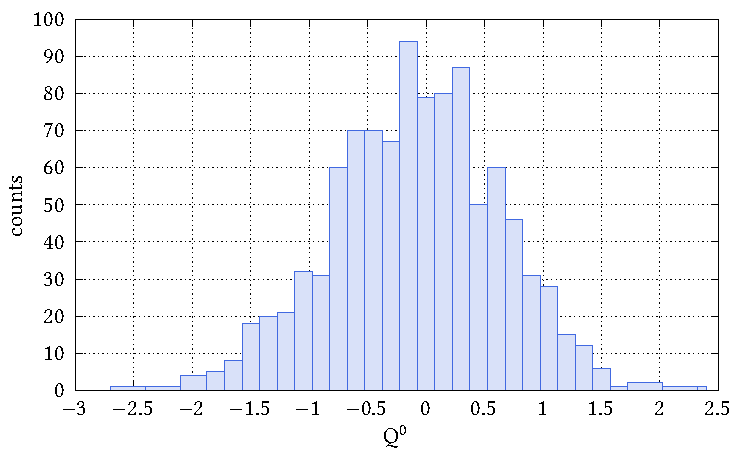
\includegraphics[width=\linewidth]{16/histo0}
  \caption{\label{fig:histo0}$Q$ at flow time $0$.}
  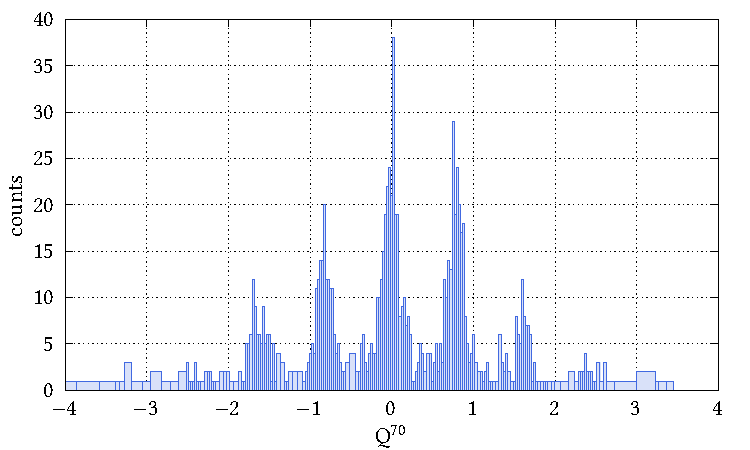
\includegraphics[width=\linewidth]{16/histo70}
  \caption{\label{fig:histo70}$Q$ at flow time $70 = \frac{t_{0}}{7}$}
\end{figure}
\begin{figure}[H]
  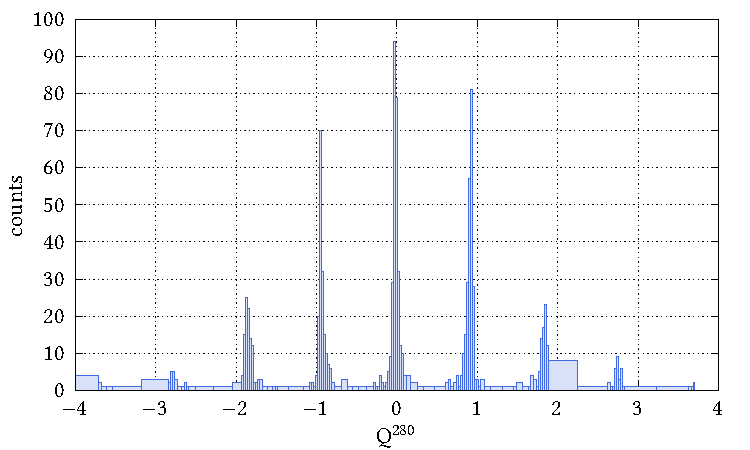
\includegraphics[width=\linewidth]{16/histo280}
  \caption{\label{fig:histo280}$Q$ at flow time $280 = 4\frac{t_{0}}{7}$}
  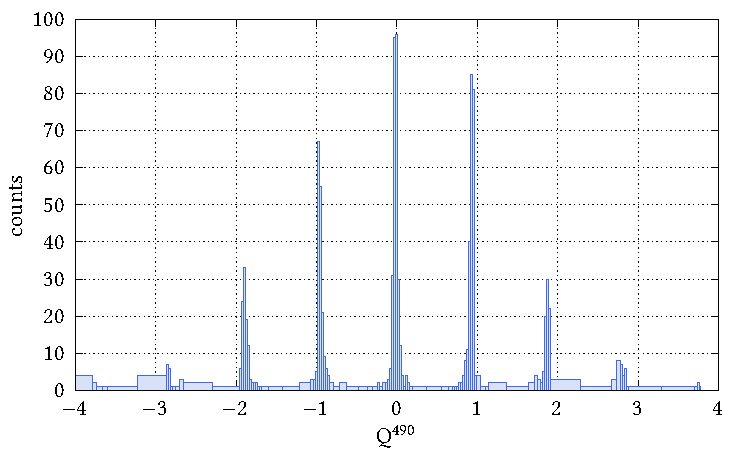
\includegraphics[width=\linewidth]{16/histo490}
  \caption{\label{fig:histo490}$Q$ at flow time $490 = t_{0}$}
\end{figure}
The values collected in table \ref{tab:values} were then plotted against $\nicefrac{a ^2}{t_{0}}$ to extrapolate the continuum limit
via a linear fit, shown in figure \ref{fig:final}. The reduced $\chi ^2$ of the fit was $\sim 10 ^{-2}$ and the continuum limit we obtained is
\begin{align}
  \label{eqn:contsusc}
  t_{0}^{2} \chi = 6.30(9)\times 10 ^{-4}.
\end{align}
\begin{figure}[H]
  \centering
  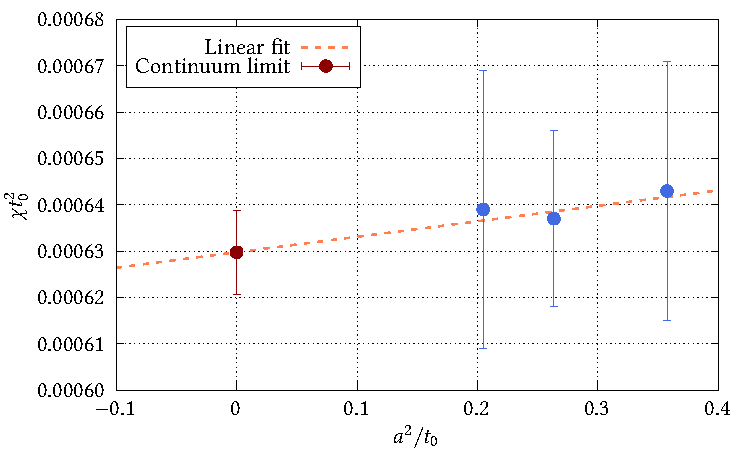
\includegraphics[width=\linewidth]{final}
  \caption{\label{fig:final}Continuum limit of $t_{0}^2\chi$. Fit performed by Gnuplot, reduced $\chi ^2\sim 10^{-2}$.}
\end{figure}
To obtain the physical value of $\chi$ we divided the fit extrapolation by $t_{0}^2$ and then converted its value from $\si{\femto\metre}^{-4}$ to
$\si{\mega\electronvolt}^{4}$, remembering the conversion rate $1\si{\femto\metre}^{-1}=\SI{197.3}{\mega\electronvolt}$. Thus, the physical value of the topological susceptibility is
\begin{align}
  \chi = \left(\SI{178(8)}{\mega\electronvolt}\right)^{4}.
\end{align}
Because of the statistical error of our measurements, we can safely input the pion leptonic decay constant $F_{\pi}$ instead of $F_{\eta'}$ inside the Witten Veneziano formula and discard
any considerations about the errors of $F_{\pi}$, $m_{K}$ and $m_{\eta}$.

Finally, using equation \ref{eqn:nonchiralmass} with the $3$ lightest quarks, we obtain the mass of the $\eta'$ meson
\begin{align}
  \label{eqn:metaprime}
  m_{\eta'} = \SI{944(69)}{\mega\electronvolt}.
\end{align}
This result deviates less than $2\sigma$ from the measured value $m_{\eta'}=958.66(24)\si{MeV}$ but comes with a $7\%$ relative error,
whose magnitude overrules any significance of the formal compatibility between the results.
Specifically, the fact that we found a smaller value for the $\eta'$ mass suggests that we underestimated the value $t_{0}^{2}\chi$.
This claim is supported by the results in \cite{Ce} where $t_{0}^{2}\chi = 6.67(7)\times 10^{-4}$, more than $3$ standard deviations away from
our extimate (equation \ref{eqn:contsusc}).
